\begin{anexosenv}


\chapter{Entrevista por Pauta}

\textbf{Entrevistado:} Leandro Luiz Fleury Rosa

\textbf{Profissão:} Optometrista

\textbf{Local:} Ótica Cristal (Goiânia)

\textbf{Pauta:}

\begin{enumerate}
\item Como surgiu a ideia ou a necessidade de um produto como esse?
\item Qual a faixa etária mais comum dos usuários de lente e possíveis usuários do produto?
\item Pela sua experiência, é grande a quantidade de pessoas que tem dificuldade de utilizar lentes? Quais pessoas possuem mais dificuldade?
\item Quais as principais características de uma lente rígida (gás permeável) e de uma lente gelatinosa? Diâmetro, textura, maliabilidade, resistência e etc.
\item Como é feita higienização ou limpeza da lente?
\item Como um dos mentores da ideia, quais as principais funcionalidades que você acredita que produto deve ter? Quais os principais benefícios?
\item Qual a sua opião sobre um processo de limpeza da lente ser integrado ao produto?
\item Existe algo que contém caracteristicas similares a um olho humano a fim de realizar testes do aparelho?
\item Explicar conceito inicial desenvolvido pela equipe para o produto e coletar opinião. 
\item Verificar possibilidade de doação de materiais.
\end{enumerate}


\chapter{Fundamentação Teórica}

\section[Instrumentação e Sensoriamento]{Instrumentação e Sensoriamento}

\subsection[Processamento de Imagens]{Processamento de Imagens}

Processamento de imagens consiste de qualquer forma de processamento de dados no qual a entrada e saída são imagens, tais como fotografia ou quadros (\textit{frames}) de algum vídeo. Geralmente esta técnica é utilizada para aprendizado de máquina ou detecção de padrões, sendo que a segunda, para este trabalho, é a mais relevante.

Na literatura consultada, são apresentadas várias técnicas de detecção de padrões com o objetivo de detectar a face e o olho em uma imagem. \citeonline{hsu} apresenta um método de detecção para ambientes onde a luz varia bastante ao longo do dia, dessa maneira o método consiste primeiramente de procurar candidatos baseando-se na cor da pele, e então através de uma análise de crominâncias, encontra-se possíveis regiões para olho, boca e nariz. 

\citeonline{huang} propuseram uma combinação de abordagens para solucionar o problema da detecção robusta de faces e olhos. Em imagens de faces de baixa resolução, os olhos e as sobrancelhas se apresentam como barras escuras que podem ser detectadas utilizando a segunda derivada de um filtro Gaussiano. Por isso aplicaram filtros Gaussianos e direcionais para detectar candidatos a olhos, sobrancelhas, boca e nariz. Após este passo, um modelo estrutural é criado para agrupar pontos característicos de candidatos à face usando relações geométricas.

Um dos algoritmos mais eficazes para a detecção de faces e olho em imagens estáticas é o algoritmo de \citeonline{viola}, que se encontra implementado na biblioteca Intel OpenCV (Intel Open Source Computer Library) e que visa localizar em uma imagem características que codifiquem alguma informação do padrão sendo detectado. Esses padrões são baseados nas características de Haar que codificam informações sobre a existência de contrastes orientados entre regiões da imagem. A Figura \ref{fig09} apresenta algumas características de Háar propostas para a detecção de faces em imagens estáticas.  


\begin{figure}[htb]
		\centering
			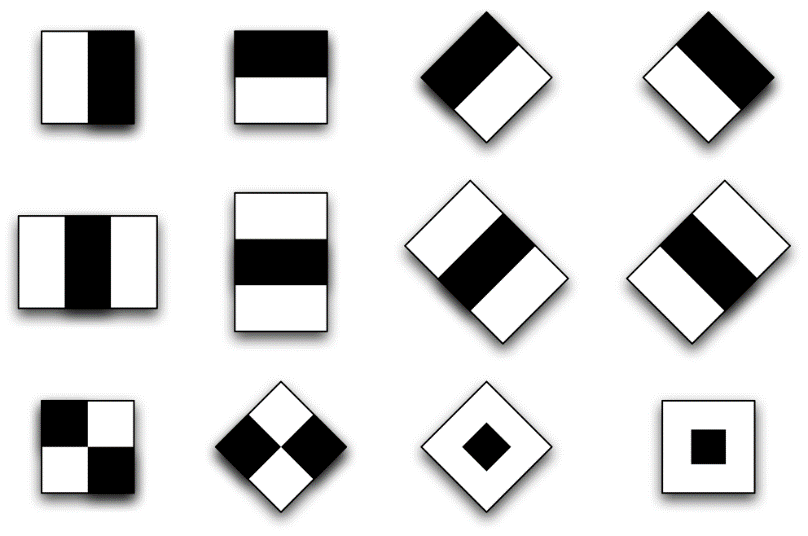
\includegraphics[scale=0.7]{figuras/haar.png}
		\caption{Características de Haar mais usadas em detecção de faces}
		\label{fig09}
\end{figure}

Quando as características de Haar são aplicadas em uma imagem, são examinados os contrastes naturais proporcionados pelas características da face, considerando suas relações de espaço, como ilustrado na Figura \ref{fig10}.


\begin{figure}[htb]
		\centering
			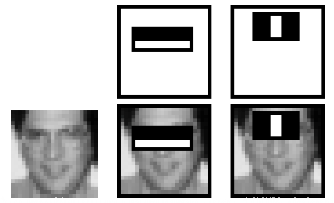
\includegraphics[scale=0.7]{figuras/haar2.png}
		\caption{Relação entre as características de Haar e os contrastes naturais da face}
		\label{fig10}
\end{figure}

De forma a complementar a detecção de possíveis regiões dos olhos através do algoritmo de Viola-Jones, é possível usar a técnica apresentada por \citeonline{hsu}, onde diz que para uma imagem no espaço de cores YCbCr, os olhos apresentam um alto valor de Cb e baixo valor para Cr. Dessa forma, ele apresenta um conjunto de operações entre o plano Cb e Cr com o objetivo de isolar as possíveis regiões de olho.

\subsection[Sensor de Proximidade Ultrassônico]{Sensor de Proximidade Ultrassônico}

Um sensor de proximidade ultrassônico possui uma alta aplicabilidade em pesquisas e indústrias. Essa alta aplicação dá-se devido a sua detecção de objetos de texturas, formas, cores e materiais diferentes, sendo assim aplicável para detecção de distancia, altura, medida de diâmetro, contagem de objetos entre outras.

Com o funcionamento baseado na emissão de ondas sonoras de alta frequência, o sensor de proximidade ultrassônico funciona medindo o tempo entre a emissão e a recepção da onda gerada pelo sensor. Esta onda, ao sair do sensor, bate no objeto que está mais próximo gerando um eco, que por sua ver volta para o sensor que é capaz de calcular a distância entre o emissor e objeto sabendo a velocidade da onda emitida e o tempo que essa onda levou para chegar novamente ao receptor, gerando assim um sinal elétrico proporcional.

\begin{figure}[htb]
		\centering
		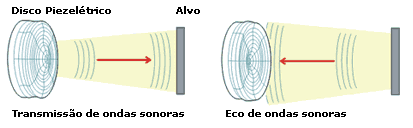
\includegraphics[scale=0.7]{figuras/sensorultra.png}
		\caption{Sensor de Proximidade Ultrassônico}
		\label{fig11}
\end{figure}

Como o espalhamento das frentes de onda destes sensores têm forma cônica, eles podem ser ajustados de maneira que o cone alcance maior distância e precisão para detecção de um determinado objeto (Fig. \ref{fig11}).

A maioria dos sensores comercializados hoje pela indústria eletrônica são capazes de detectar objetos a distancias entre 2 cm a 450 cm com uma precisão de 3 mm. Esses objetos não precisam necessariamente estarem parados na frente do sensor devido a alta velocidade de propagação da onda emitida, sendo o seu uso possível em processos de fabricação contínuos que utilizam esteiras.
 
\subsection[Sensor de Toque]{Sensores de Toque}

Sensores de toque são basicamente transdutores com sensibilidade para força, pressão ou toque humano. Esses tipos de sensores são bastante utilizados nos dias atuais, visto que os mesmos estão presentes em aplicações do tipo \textit{touch screen}, muito comum em \textit{tablets}, \textit{smartphones}, agências bancárias, \textit{notebooks}, etc.

O primeiro sensor de toque foi desenvolvido em 1971 pelo fundador da Elographics Dr. Sam Hurst e, ainda durante a década de 90, teve sua adoção disseminada com a criação dos \textit{smartphones} e demais equipamentos que utilizam a tecnologia \textit{touch screen}, como ATMs e sistemas de pontos de vendas. O uso da tecnologias \textit{touch} disseminou rapidamente quando o iPhone introduziu as habilidades de múltiplos toques e zoom utilizando estes tipos de sensores \cite{mathas}.

Os principais tipos existentes de sensores de toques são os resistivos, capacitivos, infravermelhos, e de superfície acústica (SAW, do inglês \textit{Surface Acoustic Wave}). Cada um deles podendo detectar o toque de uma forma diferente e, em alguns casos, podendo detectar gestos sem contato direto \cite{mathas}.

No presente projeto, o estudo dos sensores de toque será focado para avaliar se este tipo de sensor é apropriado para fornecer uma medida altamente precisa do momento em que a ventosa, com ou sem a lente, encosta no globo ocular do usuário da máquina. 

Devido a característica do projeto, as habilidades de zoom ou múltiplos toques que podem ser obtidos com esses sensores são irrelevantes. Apenas é necessário apontar características como sensibilidade, precisão, robustez, tamanho e custo, para saber se a medida é confiável para controlar a proximidade e toque com o olho, se o sensor é pequeno e robusto o suficiente para não apresentar falhas e ser fácil de integrar com o projeto mecânico do protótipo e se o mesmo possui custo baixo visando tornar o preço do produto final e do protótipo mais acessível. Sendo assim, as características que serão apresentadas abaixo abordarão os requisitos supracitados.

\subsubsection[Princípios de Funcionamento]{Princípios de Funcionamento}

Antes de focar nas características listadas anteriormente, é válido conhecer o princípio de funcionamento dos mesmos, de modo a restringir a pesquisa futura somente nos que realmente sejam relevantes para o projeto.



Os sensores de toque capacitivo são baseados em perturbações elétricas. Os sensores deste tipo são constituídos por lâminas de vidros que possuem um revestimento condutor de um lado e um padrão de circuito impresso ao redor da área de visualização. Basicamente, o padrão de circuito impresso cria uma carga em toda superfície do sensor, que é perturbada quando se toca com o dedo, luva ou qualquer outro objeto na tela do sensor \cite{mathas}. Conforme pode ser visualizado na Fig. \ref{fig12}.

O dedo ou qualquer outro objeto aterrado serve como uma fonte de excitação que, quando encostado na superfície metálica da lâmina de vidro, gera uma perturbação no campo elétrico que será transmitido para o padrão de circuito impresso. Tal perturbação passa por um conversor ADC (\textit{Analog to Digital Converter}) para ser, posteriormente, tratada no domínio digital \cite{ad7142} como mostra a Figura \ref{fig12}.

A interferência no campo elétrico induzido é gerada pelo desvio de linhas de campo elétrico que são desviadas para a terra e não atingem o receptor. Desta forma, ocorre uma diminuição da capacitância total medida pelo receptor\cite{ad7142} de acordo com a lei da capacitância:

$$ C = \frac{Q}{V} $$

Por serem construídos sobre o vidro, não é necessário muita pressão para obter resposta desse tipo de sensor de forma que a força é insignificante. A única desvantagem é que esses sensores são vulneráveis à abrasão do revestimento condutor \cite{mathas}.

De todos os tipos de sensores de toque este é o único que permite a tecnologia de múltiplos toques e, por isso, é muito utilizado em \textit{smartphones}, porém a utilização deste tipo de sensor tem aumentado em para aplicações industriais, médicas, automotivas e de consumo \cite{mathas}. 

\begin{figure}[htb]
		\centering
			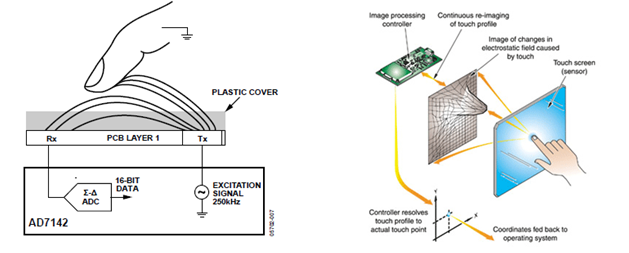
\includegraphics[scale=0.7]{figuras/sensortoque.png}
		\caption{Sensor de Toque}
		\label{fig12}
\end{figure}




O sensor de toque resistivo consiste em duas camadas que não estão em contato e separadas por um espaço bem fino. Quando ocorre uma pressão causada pelo toque, essas camadas se tocam modificando a resistência do conjunto e causando uma resposta do sensor, confirma mostra a Figura \ref{fig13} \cite{keyur}.

\begin{figure}[htb]
		\centering
			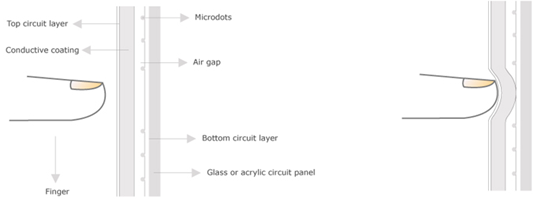
\includegraphics[scale=0.7]{figuras/variacao.png}
		\caption{Variação de Resistência}
		\label{fig13}
\end{figure}

Este tipo de sensor é a forma mais comum de sensores de toque existentes sendo usados para aplicações de distância e pressão. Em geral, este tipo de sensor é mais simples e barato. Suas limitações consistem em uma falha ocasionada pela falta de flexão necessária para empurrar o conjunto de superfícies, a redução do brilho que atravessa este sensor (queda de 10\% a 20\%) e o fato de não suportar múltiplos toques \cite{mathas}.

Este tipo de sensor oferece um custo benefício bom, leituras consistentes, desempenho durável em ambientes onde é necessário suportar contaminantes e líquidos tais como restaurantes fábricas e hospitais. Estes sensores, em geral, são muito utilizados em \textit{gadgets} e aplicações de consumo portátil \cite{mathas}.



Já os sensores de toque infravermelho trabalham com uma face de vidro em frente do LCD. Existem emissores de luz infravermelha e sensores nas quatro direções de observação, onde esses emissores ficam constantemente enviando feixes de luz infravermelha. Quando ocorre o toque, os feixes de luz são interrompidos ou alterados, o que é perceptível pelos sensores, conforme mostra a Figura \ref{fig14} \cite{vicki}. Dessa forma a pressão do toque e o objeto utilizado para efetuar o toque são irrelevantes, este tipo de sensor é mais comum de ser utilizado em aplicações envolvendo jogos e quiosques de informação \cite{mathas}.


\begin{figure}[htb]
		\centering
			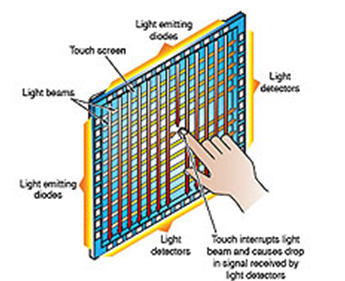
\includegraphics[scale=0.7]{figuras/infra.png}
		\caption{Sensor de Toque Infravermelho}
		\label{fig14}
\end{figure}



O funcionamento do sensor SAW, por sua vez é bastante similar ao dos sensores de toque infravermelho. A diferença consiste que, em vez de feixes de luz, serão emitidos impulsos ultrassônicos gerados por cristais piezelétricos. Estes cristais são ligados no vidro da superfície para criar os impulsos de som que se deslocam ao longo da superfície. Nesta configuração, é necessária a presença de refletores que redirecionam o som de volta aos cristais que, por sua vez, convertem as ondas mecânicas em energia elétrica \cite{mathas}.  

Quando ocorre um toque, parte do som é absorvida ou redirecionada, e assim é possível através de alguns sensores, calcular a posição onde se foi realizado o toque. Em geral esse tipo de sensor é utilizado em caixas eletrônicos, quiosques de informação e parques de diversões \cite{mathas}.

Através do principio de funcionamento dos sensores mencionados acima, é possível verificar que os sensores de toque infravermelho e SAW são mais apropriados para aplicações que envolvam uma interação com usuário através da tecnologia \textit{touch screen}. Para o sensoriamento que se deseja neste projeto, a utilização de sensores de toque capacitivos ou resistivos se torna mais adequada.

Desta forma foi levantado alguns modelos comerciais destes dois tipos de sensores visando principalmente verificar características como o tamanho do sensor, robustez, precisão, sensibilidade e preço.

\subsubsection[Modelos Comerciais]{Modelos Comerciais}

A Figura \ref{fig15}  relaciona modelos comerciais de sensores de toque capacitivos e resistivos com suas respectivas características. Devido a questões práticas, de aquisição de material, buscaram-se os sensores da marca freescale semiconducter, devido a mesma possuir diversos distribuidores localizados no Brasil.
	
Devido ao principio de funcionamento dos sensores resistivos e capacitivos, eles possuem sempre uma alta sensibilidade ao toque, e uma alta precisão para detectar o momento do toque. Quanto a robustez é válido lembrar que o sensor resistivo pode apresentar falhas referentes a flexão ocasionada pelo toque na lâmina e que o sensor capacitivo pode vir a sofrer abrasão do revestimento condutor. Desta forma será listado alguns modelos, o tipo do modelo, tamanho e custo.

\begin{figure}[htb]
		\centering
			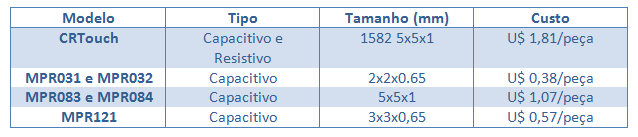
\includegraphics[scale=1.0]{figuras/toquecomerciais.png}
		\caption{Sensores de toques disponíveis no site da freescale semiconducter para venda \cite{free}.}
		\label{fig15}
\end{figure}


\subsection[Sensores de Pressão]{Sensores de Pressão}

Sensores são dispositivos projetados para detectarem algum evento no processo e emitirem um sinal de resposta a esse evento \cite{geomar}. É a parte sensitiva de um transdutor, que é um sistema que transforma duas formas de energia para fins de medida \cite{werneck}.

A pressão é uma força por uma unidade de área que um corpo exerce sobre o outro. As unidades comuns dos sensores de pressão são psi [$lb/pol^2$] e Pa [$N/m^2$]. As medidas de pressão são feitas para gases e líquidos.

A ideia básica para que o dispositivo pegue a lente do seu estojo e a mantenha na ventosa é trabalhar com pressão negativa para sucção da lente. A ventosa citada já é vendida no mercado e funciona justamente para auxiliar pessoas com dificuldade na manipulação de lentes de contato. No contexto deste projeto, vê-se a necessidade de monitorar a pressão no interior da ventosa, para que esta pressão não ultrapasse um limiar ideal de seguridade.

Os valores normais de pressão intraocular estão compreendidos entre 10 e 21 mmHg aproximadamente \cite{andre}. Os sensores serão, então, avaliados principalmente pelo range citado, precisão, sensibilidade, robustez.

\subsubsection[Princípio de Funcionamento]{Princípio de Funcionamento}

Os sensores de pressão são compostos por duas partes: a conversão de pressão em uma força ou deslocamento e conversão de força e deslocamento em sinal elétrico \cite{geomar}.

Os sensores de pressão podem ser classificados em três tipos, de acordo com a referência utilizada para a leitura \cite{patsko}:
\begin{itemize}
\item Sensores de pressão \textit{Gauge}: medem a pressão de interesse em relação à pressão atmosférica local;
\item Sensores de pressão diferencial: medem a diferença de pressão entre dois pontos distintos no circuito, onde nenhum deles está na pressão atmosférica necessariamente. Possui duas entradas de ar e o nível de tensão da saída indica a diferença entre as pressões;
\item Sensores de pressão absoluta: medem a pressão de interesse em relação em relação ao vácuo total (0 psi).
\end{itemize}

Os sensores de pressão são, dentre outros métodos, geralmente construídos com materiais piezoresistivos. Esses materiais possuem a capacidade de variar sua resistência  quando submetidos a um esforço mecânico. São construídas duas câmaras e entre elas é colocada uma película de material piezoresistivo, como ilustrado na figura \ref{fig16}. O modo como essas câmaras são construídas é que define qual é o tipo do sensor. Em um sensor de pressão absoluta, uma dessas câmeras é fechada e outra é aberta, destinada à pressão a ser medida. A câmara fechada contém vácuo, ou seja, a pressão a ser monitorada é medida em relação à pressão zero. Esse sensor é ideal para medir pressões baixas, menores do que a atmosférica \cite{patsko}.

Num sensor \textit{Gauge}, as duas câmaras são abertas, sendo que uma é destinada a pressão a ser medida, enquanto que outra é destinada a entrada de ar atmosférico. Desse modo, a pressão é medida em relação à pressão atmosférica local. Caso a pressão externa seja igual à utilizada como referência para o sensor, a força resultante sobre o material piezoresistivo será nula. Se uma das pressões for maior do que a outra, temos que a película será submetida a um esforço e sua resistência irá mudar. O sensor de pressão diferencial também possui as duas câmaras abertas, porém elas são destinadas às pressões que serão comparadas pelo sensor \cite{patsko}. Os valores comerciais dos sensores piezoresistivos são nas faixas de 0 a 1,5 psi e 0 a 5000 psi \cite{geomar}.

Nos modelos de sensores piezoresistivos, a estrutura é construída utilizando a tecnologia MEMS, que possibilita a sua montagem em dimensões extremamente reduzidas, possibilitando a integração de todos os componentes numa única peça.

\begin{figure}[htb]
		\centering
			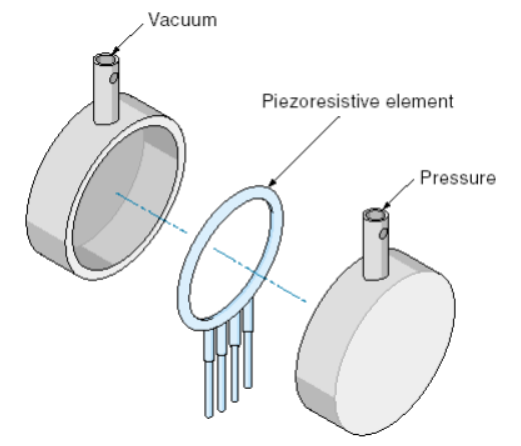
\includegraphics[scale=0.7]{figuras/sensorpressao.png}
		\caption{Sensores de pressão a semicondutor \cite{geomar}.}
		\label{fig16}
\end{figure}

O tubo de Bourdon é um medidor de pressão de grande importância no âmbito industrial, sendo uma das soluções mais utilizadas. O funcionamento deste tipo de manômetros é baseado na alteração da curvatura originada num tubo de secção elíptica pela pressão exercida no seu interior. A secção elíptica tende para uma secção circular com o aumento da pressão no interior do tubo levando a que o tubo se desenrole. Este tubo tem a uma das extremidades fechadas e ligada a um mecanismo, com rodas dentadas e mecanismos de alavanca, que permite transformar o seu movimento de "desenrolar", originado pelo aumento de pressão no interior do tubo, no movimento do ponteiro do manômetro \cite{bourdon}. O tubo de Bourdon é disponível para pressões de 30 a 100.000 psi \cite{geomar}.

\begin{figure}[htb]
		\centering
			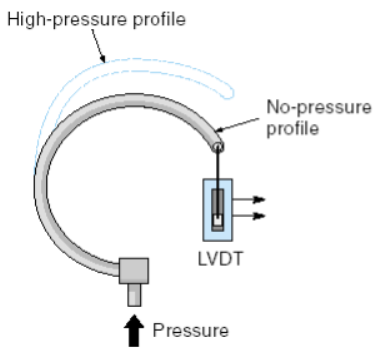
\includegraphics[scale=0.7]{figuras/bourdon.png}
		\caption{Ilustração do tubo de Bourdon. Um sensor de posição , como um LVDT, transforma o deslocamento em um sinal elétrico \cite{geomar}.}
		\label{fig17}
\end{figure}

\subsubsection[Modelos comerciais]{Modelos comerciais}

São apresentados  na figura \ref{fig18} alguns modelos comerciais de sensores de pressão que podem ser utilizados na prototipação do projeto. Como a pressão do olho é de 10 a 21mmHg, 1,3Kpa a 2,8KPa os sensores cabíveis são os com princípio piezoresistivo.

\begin{figure}[htb]
		\centering
			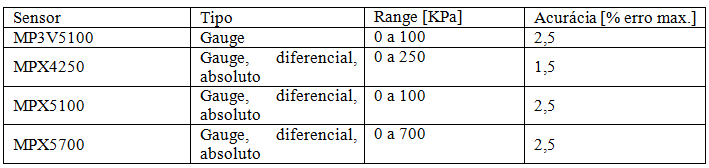
\includegraphics[scale=0.8]{figuras/pressaocomerciais.png}
		\caption{Modelos comerciais de sensores cabíveis ao projeto \cite{free2}.}
		\label{fig18}
\end{figure}







\section[Controle e Atuação]{Controle e Atuação}

\subsection[Atuadores]{Atuadores}

Em um sistema, atuador é um elemento que atende a comandos do controlador e produz movimento. Em linhas gerais, o atuador transforma algum tipo de energia de entrada em movimentos, que pode ser considerado energia cinética. Os atuadores podem ter seu movimento induzido por força de origem pneumática, hidráulica, elétrica, combustão ou até mesmo por deformação termal de materiais \cite{machado}.

Ainda, os atuadores podem fornecer basicamente dois tipo de movimento: 1) rotativo: como é o caso dos motores e; 2) linear (ou translação): como é o caso dos pistões e solenoides que podem oferecer um avanço ou recuo. A escolha do atuador deve ser feita a partir deste requisito inicial, contudo, é possível converter um tipo de movimento no outro. Para converter um movimento rotativo em linear, pode-se utilizar um sistema de pinhão e cremalheira ou eixo acoplado a rosca sem fim. Para converter um movimento linear em rotativo, pode-se utilizar o sistema de biela e eixo assimétrico, como o existente nos motores dos veículos \cite{machado}.

Os atuadores rotativos ainda podem ser classificados em:
\begin{itemize}
	\item angulares: quando giram apenas num ângulo limitado, como é o caso dos servomotores e motores de passo;
	\item contínuos: que têm a possibilidade de realizar número indeterminado de rotações, como é o caso dos motores de corrente contínua.
\end{itemize}

Tal como o nome sugere, um servomecanismo deve obedecer a comandos. Sendo este geralmente interligado a um sistema de malha fechada com realimentação, ele informa ao controlador se a tarefa foi executada. O controlador monitora a atuação do servomecanismo e através de sensores de posição e compensa eventuais discrepâncias entre o valor desejado e o valor obtido \cite{SCME}.



\subsubsection[Tipos de Atuadores]{Tipos de Atuadores}

Será feita adiante uma breve explicação sobre cada tipo de atuador existente, explicitando suas características genéricas e pontuando quais tipos são mais adequados para este projeto.

\textbf{Motores Elétricos de Corrente Contínua (CC)}

Os motores elétricos são máquinas elétricas que caracterizam atuadores do tipo rotativo e podem ser subdivididos em motores angulares ou de rotação contínua. 

Em se tratando de aspectos construtivos, o motor CC pé composto por duas estruturas magnéticas \cite{siemens}:
\begin{itemize}
	\item Estator (enrolamento de campo ou imã permanente)
	\item Rotor (enrolamento de armadura)
\end{itemize}

O estator é composto de um imã permanente ou de uma estrutura ferromagnética onde são enroladas bobinas que formam o campo. Já o rotor é um eletroímã  constituído de um núcleo de ferro com enrolamentos em sua superfície que são alimentados por um sistema mecânico de comutação como mostra a Figura \ref{estruturamotor}.

\begin{figure}[htb]
		\centering
			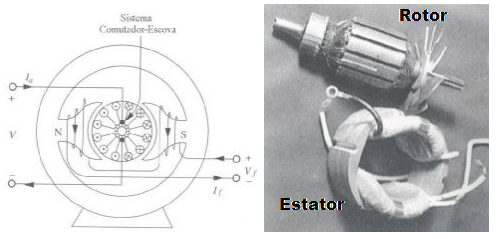
\includegraphics[scale=0.9]{figuras/estruturamotorcc.png}
		\caption{Estrutura de um motor CC \cite{siemens}}
		\label{estruturamotor}
\end{figure}

Quanto ao seu tipo de configuração de enrolamentos, podem ser classificados de acordo com o organograma da Figura \ref{fig19} \cite{siteeducation}:

\begin{figure}[htb]
		\centering
			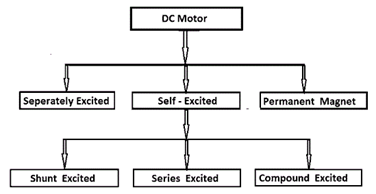
\includegraphics[scale=0.9]{figuras/motores1.png}
		\caption{Classificação dos motores quanto ao tipo \cite{siteeducation}}
		\label{fig19}
\end{figure}

Os motores de corrente alternada (CA) não aparecem na figura acima, pois não são recomendados para aplicações de baixa potência onde prevalece o controle de pequenos sinais elétricos. Dependendo da aplicação, os acionamentos em corrente contínua são geralmente os que apresentam os maiores benefícios, também em termos de confiabilidade, operação amigável e dinâmica de controle. Assim, podemos enumerar algumas vantagens \cite{siemens}:
\begin{itemize}
	\item Operação em 4 quadrantes com custos relativamente mais baixos; 
	\item Ciclo contínuo mesmo em baixas rotações;
	\item Alto torque na partida e em baixas rotações;
	\item Ampla variação de velocidade;
	\item Facilidade em controlar a velocidade;
	\item Os conversores CA/CC requerem menos espaço;
	\item Confiabilidade;
	\item Flexibilidade (vários tipos de excitação);
	\item Relativa simplicidade dos modernos conversores CA/CC.
\end{itemize}

E desvantagens:
\begin{itemize}
	\item Os motores de corrente contínua são maiores e mais caros que os motores de indução, para uma mesma potência;
	\item Maior necessidade de manutenção (devido aos comutadores);
	\item Arcos e faíscas devido à comutação de corrente por elemento mecânico (não pode ser aplicado em ambientes perigosos);
	\item Tensão entre lâminas não pode exceder 20V, ou seja, não podem ser alimentados com tensão superior a 900V, enquanto que motores de corrente alternada podem ter milhares de volts aplicados aos seus terminais;
	\item Necessidade de medidas especiais de partida, mesmo em máquinas pequenas (uso de \textit{soft starters}.
\end{itemize}

A classificação dos motores de corrente contínua é dada de acordo com o tipo de excitação de seus enrolamentos do campo e da armadura. A Figura \ref{fig20} mostra a configuração dos enrolamentos de cada tipo de motor CC \cite{siteeducation}.

\begin{figure}[htb]
		\centering
			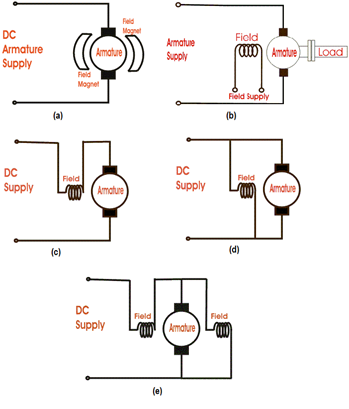
\includegraphics[scale=0.9]{figuras/motores2.png}
		\caption{Tipos de motores de corrente contínua: a) motor de imã permanente; b) motor de excitação separada; c) motor de excitação série; d) motor de excitação shunt; e) motor de excitação mista \cite{siteeducation}}
		\label{fig20}
\end{figure}

Cada tipo de configuração apresenta características diferentes de acordo com o que se segue \cite{siemens}:

\par \vspace{\baselineskip}
\par \vspace{\baselineskip}

\noindent
Motor de excitação em série:
\begin{itemize}
	\item Bobinas de campo estão em série com o  enrolamento da armadura;
	\item Só há fluxo no entreferro da máquina quando a corrente da armadura for diferente de zero;
	\item Conjugado elevado em baixa rotação;
	\item Potência constante;	
	\item Velocidade extremamente elevada quando o motor é descarregado.
\end{itemize}

\noindent
Motor de excitação em paralelo (shunt):
\begin{itemize}
	\item Velocidade praticamente constante;
	\item Velocidade ajustável por variação da tensão de armadura.
\end{itemize}

\noindent
Motor de excitação independente:
\begin{itemize}
	\item Motor excitado externamente pelo circuito de campo;
	\item Velocidade praticamente constante;
	\item Velocidade ajustável por variação da tensão de armadura e também por enfraquecimento de campo;
\end{itemize}

\noindent
Motor de excitação composta:
\begin{itemize}
	\item Enrolamento de campo independente;
	\item Apresenta um fluxo mínimo mesmo com o motor em vazio.
\end{itemize}

Em geral, os motores de corrente contínua, quando acionados, giram de forma contínua e ininterrupta. O sentido de rotação é dado pela polaridade da tensão de excitação da armadura e para inverter o sentido de giro se faz necessário um circuito chamado de ponte-H. A Figura \ref{fig21} mostra um motor de corrente contínua.

\begin{figure}[htb]
		\centering
			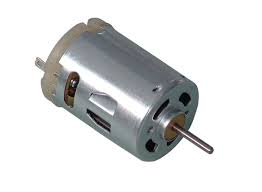
\includegraphics[scale=0.9]{figuras/motores3.png}
		\caption{Motor de corrente contínua}
		\label{fig21}
\end{figure}




\textbf{Motores de Passo}

Os motores de passo configuram boas escolhas em aplicações que necessitam controlar ângulo de rotação, velocidade, posição e sincronismo. A maior vantagem deste tipo de motor está na possibilidade de controlar seus movimentos com precisão. Por conta disso, ele é amplamente utilizado em impressoras, scanners, robôs, câmeras de vídeo, entre outros dispositivos \cite{brites}. Uma de suas desvantagens é que ele pode "pular" passos, caso a carga no eixo seja muito grande e, a menos que se tenha um dispositivo que controle sua rotação, não é possível compensar estes "pulos". Outra desvantagem é que eles causam mais ruído e vibração que os outros tipos de motores \cite{nippon}. A figura \ref{motordepasso} mostra um motor deste tipo.

\begin{figure}[H]
		\centering
			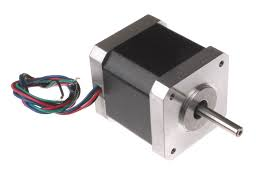
\includegraphics[scale=1.0]{figuras/motordepasso.png}
		\caption{Motor de passo}
		\label{motordepasso}
\end{figure}

O acionamento deste motor também necessita de um circuito especial que possa acionar cada bobina individualmente. Os motores de passo bipolares (Figura \ref{bipolar}) possuem apenas um enrolamento por fase. Para fazer o acionamento sequencial destes enrolamentos, necessita-se efetuar os seguintes acionamentos sequenciais e de forma cíclica: 
\begin{enumerate}
\item Polarizar a fase 0 durante alguns milissegundos; 
\item Despolarizar a fase 0;
\item Polarizar a fase 1 durante alguns milissegundos;
\item Despolarizar a fase 1;
\item Polarizar a fase 0 reversamente durante alguns milissegundos;
\item Despolarizar a fase 0;
\item Polarizar a fase 1 reversamente durante alguns milissegundos;
\item Despolarizar a fase 0.
\end{enumerate}

Esta sequência pode ser repetida inúmeras vezes enquanto se desejar que o motor mantenha-se em rotação. Caso deseje-se que o motor fique travado na posição atual, basta deixar um dos enrolamentos energizados. Se todos os enrolamentos ficarem desligados, o eixo do rotor fica livre. E se a sequência for invertida, o sentido de rotação do motor também é invertido.

Quanto menor o tempo em que as bobinas ficam energizadas, maior será a velocidade de rotação do motor. Porém, existe um limite mínimo de tempo que os enrolamentos necessitam ficar energizados. Caso este limite não seja respeitado, o motor não irá girar corretamente.

Por se fazer necessário que os enrolamentos sejam polarizados em dois sentidos diferentes, este motor também precisa de um circuito de ponte-H para cada enrolamento. Esta, com certeza, é uma das maiores desvantagens deste tipo de motor, pois além de necessitar de uma lógica que controle a sequência dos pulsos nos enrolamentos, ainda necessita de um circuito de ponte-H que pode ser bastante volumoso e dispendioso.

\begin{figure}[H]
		\centering
			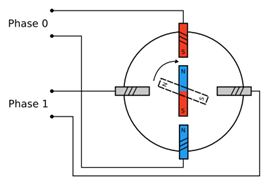
\includegraphics[scale=1.0]{figuras/bipolar.png}
		\caption{Enrolamentos de um moto de passo bipolar}
		\label{bipolar}
\end{figure}

No caso dos motores de passo unipolares (Figura \ref{unipolar}), existem dois enrolamentos por fase (enrolamentos com derivação central). Com isto, não se faz necessário a inversão da corrente em cada enrolamento, sendo dispensável o uso de uma ponte-H.

\begin{figure}[H]
		\centering
			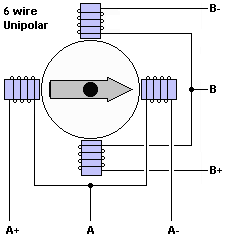
\includegraphics[scale=1.0]{figuras/unipolar.png}
		\caption{Enrolamentos de um motor de passo unipolar}
		\label{unipolar}
\end{figure}

Neste tipo de motor, os pontos A e B pode ser ligados ao VCC do circuito e a sequência de acionamento será:
\begin{enumerate}
\item Conectar ao GND o enrolamento A+ por alguns milissegundos;
\item Desconectar o enrolamento A+;
\item Conectar ao GND o enrolamento B- por alguns milissegundos;
\item Desconectar o enrolamento B-;
\item Conectar ao GND o enrolamento A- por alguns milissegundos;
\item Desconectar o enrolamento A-;
\item Conectar ao GND o enrolamento B- por alguns milissegundos;
\item Desconectar o enrolamento B-.
\end{enumerate}




\textbf{Servomotores}

Ainda existe uma terceira classe de motores elétricos que são os servomotores. Eles nada mais são que motores de corrente contínua com encoders ou potenciômetros embutidos e acoplados ao seus rotores. Os encoders e os potenciômetros servem para controlar de forma bastante precisa a velocidade e a posição do motor, respectivamente. A figura \ref{fig24} mostra um motor com encoder embutido.

\begin{figure}[htb]
		\centering
			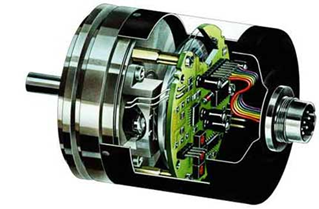
\includegraphics[scale=0.9]{figuras/motores6.png}
		\caption{Servomotor}
		\label{fig24}
\end{figure}

Devido a esta configuração, os servomotores são considerados dispositivos de malha fechada (Figura \ref{closedloop}), controlados dinamicamente por um circuito integrado à estrutura do mesmo. Isto trás uma vantagem imensa, pois se uma carga muito pesada for acoplada ao seu eixo, o controlador irá aumentar a corrente de enrolamento para que o motor movimente-se na velocidade desejada ou para a posição desejada. Em contrapartida, dependendo de suas especificações, estes motores podem custar muito caro \cite{nippon}.

% \begin{figure}[htb]
% 		\centering
% 			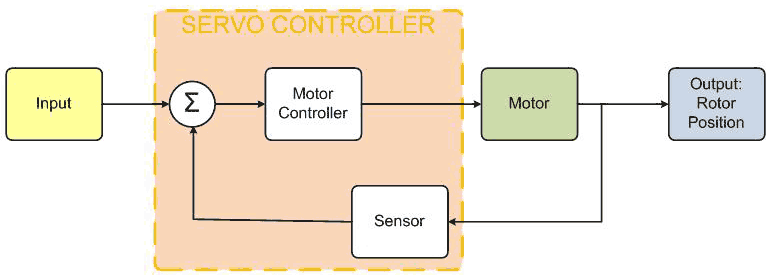
\includegraphics[scale=0.6]{figuras/closedloop.png}
% 		\caption{Realimentação em malha fechada de um servomecanismo}
% 		\label{closedloop}
% \end{figure}





\textbf{Solenoides}

Solenoides são componentes eletromecânicos e são basicamente constituídos de um fio de cobre esmaltado enrolado em volta de um carretel. O carretel é uma peça cilíndrica com seu interior oco e dentro deste espaço vazio é posicionado um êmbolo de material ferromagnético. Este êmbolo ainda é acoplado a uma mola. Quando a bobina é energizada, ela cria um campo magnético que atrai o êmbolo para dentro do carretel e comprime a mola. Quando a bobina é desligada, a mola restaura a posição inicial do êmbolo (vide Figura \ref{solenoide}).

\begin{figure}[htb]
		\centering
			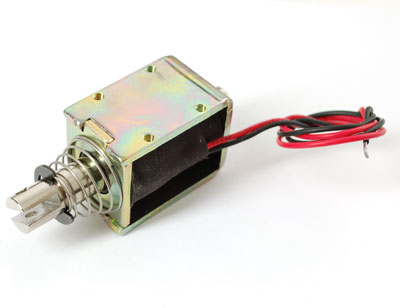
\includegraphics[scale=0.6]{figuras/solenoide.png}
		\caption{Solenoide}
		\label{solenoide}
\end{figure}

Este dispositivo possui apenas dois estados: ligado ou desligado. Ele produz um movimento linear, todavia não é possível controlar a velocidade deste movimento e é sabido que ele gera um solavanco forte acompanhado de ruído sonoro. Além disto, uma bobina consome muita energia e aquece consideravelmente. Estes aspectos podem limitar muito sua utilização \cite{machado}.




\textbf{Pistões}

Pistões, também conhecidos como cilindros, são componentes que produzem movimentos lineares e podem ter acionamento de caráter pneumático ou hidráulico. Um fluxo de ar ou de líquido, inserido na câmara interna do cilindro, movimenta o êmbolo e o faz deslocar-se até uma determinada posição. Quando o fluido é retirado da câmara do cilindro, o êmbolo retorna.

Apesar do movimento do êmbolo de um pistão ser mais suave, o controle de sua posição é impreciso.

\begin{figure}[htb]
		\centering
			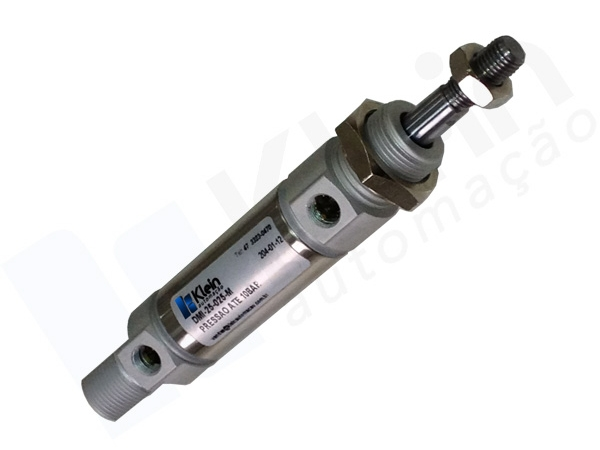
\includegraphics[scale=0.6]{figuras/pistao.png}
		\caption{Pistão}
		\label{pistao}
\end{figure}



\section[Integração e teste]{Integração e teste}

A literatura sobre Integração Interfuncional sugere que departamentos devem buscar se relacionar de modo a aprimorar resultados do processo de produção. Contudo, descrevendo de modo geral, os gerentes de cada departamento têm experimentado relações por algumas vezes conflituosas e motivadas pela busca de objetivos individuais. Observa se que,  por esse e outros motivos, o desempenho conjunto das áreas internas como um todo acaba por ser prejudicado. Parte das soluções para esses problemas apontam para o aperfeiçoamento dos mecanismos de integração dos processos de produção e para os testes e validações dos módulos individuais e agrupados que darão forma ao produto final.

\subsection[Repetibilidade]{Repetibilidade}

A repetibilidade de um dado processo ou instrumento diz respeito a aproximação de medições sucessivas de um mesmo objeto de estudo efetuadas sob as mesmas condições de medição. Estas condições são designadas por condições de repetibilidade, que incluem: o mesmo procedimento de medição, usado nas mesmas condições; o mesmo observador; o mesmo instrumento de medição, utilizado sob as mesmas condições; o mesmo local; a repetição deve realizadas em curto espaço de tempo \cite{aurelio}. 

Para garantir a confiabilidade e a qualidade do produto, faz-se uso dos conceitos de repetibilidade para a homologação das características operacionais de cada módulo e consequentemente do sistema. A exatidão dos valores obtidos a partir de diferentes ensaios está diretamente ligada a gerência dos recursos de teste de sistema – conhecimento em processos de testes, calibração dos equipamentos de teste e dos sensores e transdutores do sistema, correto registro das respostas e resultados experimentais.

\subsection[Exequibilidade]{Exequibilidade}

A exequibilidade deve ser medida pela capacidade de desenvolvimento do projeto, independente de fatores de concessão financeira. O projeto torna se exequível quando se é capaz de se obter alternativas próprias para o desenvolvimento. Um projeto também se torna exequível, quando apresenta diagnósticos das necessidades e possui aprovação da comunidade. No contexto, do projeto do Colocador de Lentes o conceito de exequibilidade foi aplicado a todas as decisões, pois é de fundamental importância que o produto e o processo de produção fossem totalmente exequíveis.

\subsection[Teoria da Confiabilidade: definição e discussões]{Teoria da Confiabilidade: definição e discussões}

Baseado na teoria de \citeonline{martin} e \citeonline{norman}, o advento da microeletrônica modificou profundamente as relações politicas, sociais e econômicas em nossa sociedade, tornando-nos dependentes de sistemas eletrônicos e computacionais. O desenvolvimento de microprocessadores em tamanhos mínimos possibilitou a utilização de sistemas operacionais de alta complexidade em dispositivos tais como celulares, câmeras fotográficas, relógios, tablets presentes em nossas atividades diárias, modificando a maneira como nos comunicamos com o mundo e realizamos nossas tarefas. A ciência e a tecnologia demandam alto desempenho de hardware e alta qualidade em software para manter os avanços e melhoras nas pesquisas atualmente realizadas. Pode-se analisar virtualmente qualquer indústria – automotiva, aeroespacial, petróleo e gás, farmacêuticas, biomédicas – todas estas indústrias são altamente dependentes de sistemas eletrônicos e computacionais para realização de tarefas básicas e complexas.

A demanda por sistemas de hardware e software de alta complexidade cresce mais rapidamente que a habilidade de projetar, implementar, testar e manter estes sistemas. Quando os requisitos por alto desempenho aumentam, as possibilidades de falhas nos sistemas responsáveis pelo processamento aumentam concomitantemente. Tais falhas podem causar simples inconveniências, perdas financeiras e mortes, o que torna a garantia de funcionamento satisfatório dos dispositivos produzidos imprescindível. 
Para suprir as necessidades de se garantir o bom desempenho e qualidade, evitar falhas e reduzir custos, grandes empresas e centros de pesquisas aplicaram-se em desenvolver métodos quantitativos e qualitativos para análise de seus produtos. A teoria da confiabilidade utilizada no século XIX em companhias de seguro de vida e marítimos foi introduzida no ambiente industrial objetivando-se a otimização e validação de processos e produtos. 

A confiabilidade é definida na ITU – International Telecommunications Union – como “a capacidade de um item para executar uma função requerida sob dadas condições para um determinado tempo”. De acordo com esta definição, os elementos básicos da teoria da confiabilidade são probabilidade, desempenho adequado, duração do desempenho adequado e condições operacionais. Em outras palavras confiabilidade é a qualidade do produto ao longo do tempo considerando-se aspectos ambientais e temporais.

Para avaliar a confiabilidade de sistemas eletrônicos pode-se preparar um modelo baseado em modelos distintos para análise de hardware e software. O modelo de confiabilidade de hardware consiste em todos os elementos do sistema de hardware em série de modo que todos os requisitos possam ser analisados com base na taxa de falhas do equipamento. Componentes individuais de software não falham independentemente e não estão sujeitos a desgastes físicos ao longo do tempo. Componentes de software falham em associação com um perfil profissional e devem ser modelados desta maneira.

Algumas ferramentas e metodologias de análise são constantemente empregadas em processos de validação da fiabilidade de componentes e sistemas eletrônicos de baixa e alta complexidade. Tais ferramentas são utilizadas em conjunto com conceitos de análise estatística para determinação de níveis de confiabilidade dos componentes e módulos de um sistema eletrônico. Listam-se algumas metodologias mais recorrentes na literatura:

\begin{itemize}
\item Process Failure Modes and Effects Analysis (FMEA): é uma técnica estruturada para identificar, registrar e priorizar potenciais falhas em um processo ou produtos, bem como suas causas e efeitos;
\item Diagrama de Ishikawa: esta ferramenta viabiliza o diagnóstico das causas de efeitos estabelecidos. É representado por um diagrama de espinha de peixe ilustrando o problema as possíveis contribuições das causas, agrupadas nas classes: pessoas, equipamentos, materiais, métodos e ambiente (PEMME, sigla em língua inglesa);
\item Mistake Proofing: esta ferramenta é utilizada a fim de evitar que falhas ocorram. Esta metodologia é subdivida em duas categorias distintas: alarmes e controles. Alarmes notificam auditiva ou visualmente uma falha detectada. Dispositivos ou medidas de controle interrompem um processo impedindo sua continuação a um próximo estágio até que uma ação corretiva seja implementada. A chave para o valor desta técnica se assenta na utilização da FMEA a fim de agir corretivamente e eliminar as oportunidades de recorrência;
\item Quality Function Deployment (QFD): esta metodologia viabiliza a identificação, classificação e fornecer soluções para os requisitos dos clientes. Neste sentido, QFD pode ser usado para identificar quais características do processo de produção são os principais impulsionadores para se atingir a confiabilidade requisitada pelos clientes;
\item Statistical Process Control (SPC): em um ambiente de produção enxuta, SPC é considerado um elemento central da gama de ferramentas de prevenção de não-conformidade. Preocupa-se com o estabelecimento e controle dos limites aceitáveis de variação estatística para um parâmetro de saída do sistema em condições de estado estacionário. Os limites aceitáveis para a variabilidade do processo são calculados e os limites de controle apropriados são fixados. Se estes limites forem extrapolados, interrompe-se o processo e põe-se em prática medidas corretivas;
\item Design of Experiments (DoE): DoE é utilizado em planejamento de experimentos ou ensaio com múltiplas variáveis. É uma coleção de métodos estatísticos que cientistas e engenheiros utilizam para melhorar a eficiência de seus projetos. Quando utilizado corretamente minimiza o número de experimentos necessários para determinar o efeito de cada variável na saída do processo ou sistema. 
\end{itemize}

Para esse projeto, a utilização de métodos de controle e análise voltados à produção em larga escala em pesquisas científicas pode se tornar contraproducente, visto que se tem por objetivo possível implementação de um único protótipo funcional. Para as características observadas do sistema a ser implementado, as metodologias de gerenciamento e controle das qualidades de experimentos apresentam-se como opção ferramental viável para a manutenção da qualidade instrumento biomédico a ser projetado e implementado.

\end{anexosenv}
